\documentclass[12pt,includeheadfoot,a4paper]{report}
\usepackage[print,nopanel]{pdfscreen}
%\begin{print}
\usepackage{lipsum}% http://ctan.org/pkg/lipsum
\usepackage{titletoc}
%\section{type}
\usepackage{lastpage}
\usepackage{macro/macro}
\usepackage{float}
\usepackage{fancyhdr}
\usepackage{booktabs}
\usepackage{array}
\newcolumntype{K}[1]{>{\centering\arraybackslash}p{#1}}
\usepackage{xcolor, colortbl}
\definecolor{Gray}{gray}{0.85}
\usepackage{verbatim}
\usepackage[Glenn]{fncychap}
\usepackage{placeins}
\let\Oldsubsection\subsection
\renewcommand{\subsection}{\FloatBarrier\Oldsubsection}
\lhead{\bfseries OpenSCAD's customizer}
\rhead{}
\usepackage[left=2.5cm, right=1.5cm, top=1.5cm, bottom=1.5cm]{geometry}
\pagestyle{fancy}
%\end{print}
\margins{2.5cm}{1.5cm}{1.5cm}{1.5cm}
\linespread{1.25}
\screensize{8cm}{9cm}
\overlay{overlay8.pdf}
\usepackage{graphicx}


\begin{document}
	\newcommand{\centertext}[1]{\begin{center}\textbf{#1}\end{center}}
\newcommand{\student}{\vskip 2.5cm}
\newcommand{\supervisor}{\vskip 2cm}
\newcommand{\stamp}{\vskip 2.5cm}
\newcommand{\HRule}{\rule{\linewidth}{0.5mm}}
\newcommand{\projecttitle}{ \fontsize{24}{25}\selectfont \bf{3D Modeling of Watertank}}
\newcommand{\tab}[1]{\hspace{.4\textwidth}\rlap{#1}}
\newcommand{\itab}[1]{\hspace{.05\textwidth}\rlap{#1}}
\newcommand{\logo}[1]{\includegraphics[scale=0.16]{#1}}
\newcommand{\submitted}{
\vskip 0.4in
\textnormal{ {\fontsize{14}{16}\selectfont \textbf{Project Synopsis}} \\
	{\fontsize{12}{13}\selectfont of Major Project}\\
}
\vskip 0.2in

\textnormal{
 {\fontsize{14}{16}\selectfont \textbf{Bachelor of Technology}\\}
 {\fontsize{16}{17}\selectfont  (Information Technology)\\}
}
\vskip 2cm
%\image{0.7}{images/gne.png}{}

\includegraphics[width=7cm]{images/gne.png}
\vskip 2cm
\begin{minipage}{0.4\textwidth}
\begin{flushleft} \large
{Submitted by:}\\
\textnormal{{\fontsize{12}{13}\selectfont Harnarinder Singh Deol\\ D3IT 2014-18 \\146031\\1411262 \\}} % Your name
\end{flushleft}
\end{minipage}
~
\begin{minipage}{0.4\textwidth}
\begin{flushright}
\textnormal{ \\
	 {\fontsize{12}{13}\selectfont V.P.O Ranguwal Disit Ludhiana
	9814797691\\ honeydeol264@gmail.com\\                 }} % Supervisor's Name
\end{flushright}
\end{minipage}\\[1.5cm]
\HRule \\[0.4cm]

\textnormal{
Guru Nanak Dev Engineering College \\
Ludhiana 141006}
}


\newcommand{\pagetitle}{\begin{center}
\projecttitle
\Large\textbf{}\\
\submitted
\vskip 1cm

\end{center}}
\newcommand{\openoffice}{\textbf{OpenOffice}}
\newcommand{\frontmatter}[1]{\begin{Large} \textbf{#1} \end{Large}}
\newcommand{\ppttitle}{\begin{center}
\end{center}}

	\begin{screen}
		\ppttitle
	\end{screen}
\thispagestyle{empty} 
\pagetitle
\newpage
\pagenumbering{Roman}
\cfoot{\thepage}

\begin{Large}
\centertext{Abstract}
\end{Large}

CAD development project discuss the work done in computer-aided-design. Computer-aided
design (CAD) is the use of computer systems to assist in the creation, modification, analysis, or
optimization of a design.I explored OpenSCAD source code. OpenSCAD is Free and Open Source
CAD Software. OpenSCAD is a fully comprehensive 3D CAD application that you can download
and install for free. There is a large base of satisfied OpenSCAD users worldwide, and it is available
in more than 20 languages and for all major operating systems, including Microsoft Windows, Mac
OS X and Linux (De- bian, Ubuntu, Fedora, Mandriva, Suse ...). OpenSCAD is an application for
Computer Aided Design (CAD) in three dimensions (3d).
OpenSCAD is a software for creating solid 3D CAD objects. It is free software and available for
Linux/UNIX, MS Windows and Apples OS X. Unlike most free software for creating 3D models
(such as the famous application Blender) it does not focus on the artistic aspects of 3D modelling
but instead on the CAD aspects. Thus it might be the application you are looking for when you
are planning to create 3D models of machine parts but pretty sure is not what you are looking
for when you are more interested in creating computer-animated movies. OpenSCAD is not an
interactive modeller. Instead it is something like a 3D-compiler that reads in a script file that
describes the object and renders the 3D model from this script file (see examples below). This
gives you (the designer) full control over the modelling process and enables you to easily change
any step in the modelling process or make designes that are defined by configurable parameters.
Also, this project makes this Project 3D model of Water Tank.In this project, the user will be
able to enter the specifications of the Water Tank through the web browser using Django (Python
Web Framework) and on the back-end, the OpenSCAD will use those input values to Draw the
Water Tank for certain parametric and in this by filling a dimmension of a water tank by the user
on a web browser and he/she will obtain a zip file on a browser then a user can download that zip
file from a browser and unzip that file and open that file in a OpenSCAD. when this file is open
by the user in an OpenSCAD then hs to be/she has to be render that file with a function key (f5).
The output that can be taken has format .scad.
This project is completely open source and the entire code is available to the user as and when
required. There is also Complete developer’s Documentation as well as User manual along with it
that helps using it a lot easier.

\newpage
\begin{Large}
\centertext{Acknowledgement}
\end{Large}

I, student of Guru Nanak Dev Engineering College, Ludhiana, have taken efforts in this project.
However, it would not have been possible without the kind support and help of many individuals
and organizations. I would like to extend my sincere thanks to all of them.
The author is highly grateful to Dr. M.S. Saini Director, Guru Nanak Dev Engineering College,
Ludhiana for providing him with the opportunity to carry out his Six Weeks Training at Testing
and Consultancy Cell, Guru Nanak Dev Engineering College, Ludhiana.
The author would like to whole heartedly thank Dr. H.S. Rai Dean, Testing and Consultancy
Cell, Guru Nanak Dev Engineering College, Ludhiana who is a vast sea of knowledge and without
whose constant and never ending support and motivation, it would never have been possible to
complete the project and other assignments so efficiently and effectively.
Finally, I would thanks My Mentors at OpenSCAD organization blobule Without their en-
couragement and Guidence, it would not have been possible to complete this project in such an
efficient manner.

\vskip 1.0cm 
\noindent Harnarinder Singh Deol


\tableofcontents
\listoffigures
\pagenumbering{arabic}
\cfoot{\thepage}

\chapter{INTRODUCTION}
\section{Overview}
\begin{figure}[H] 
	\centering 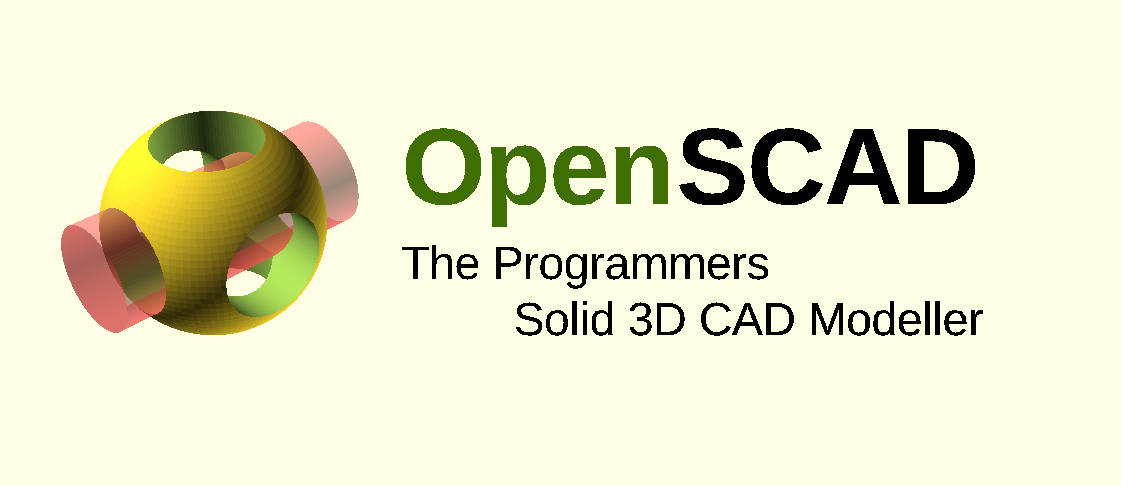
\includegraphics[scale=0.31]{images/openscad.png}
	\caption{OpenSCAD's logo}
	\label{fig:openscadlogo}
\end{figure}

User Interface for Customizing Models in OpenSCAD is the project that I worked upon it in my "Minor Project". It is under the umbrella organization of BRL-CAD. OpenSCAD is a free and Open-source software application for creating solid 3D CAD objects. It is a script only based
modeler, with a specific description language. Parts cannot be selected or modified by mouse
in the 3D view. An OpenSCAD script specifies geometric primitives and defines how they are
modified and manipulated to render a 3D model. OpenSCAD is available for Windows, Linux and
OS X. It does constructive solid geometry (CSG). OpenSCAD has in a way redefined how easy
3D modeling can be. But the Wikipedia article on OpenSCAD says that it is a non-interactive
modeler, but rather a 3D compiler based on a textual description language. Pay attention to the
above line, its primarily what Ill be talking about. Solid 3D modeling. That sounds like some
serious business. But its just an awesome tool for making models pertaining to many uses (mostly
3D printing). And 3D printing as we can all agree upon is cool. 3D models can be created by
anyone using OpenSCAD. OpenSCAD is as much for designers as it is for you and me. What
else can most people agree upon apart from the fact that solid 3D modeling is cool? A graphical
interface is simpler and more intuitive to use. There is a general aversion for typing commands in
order to get things done. Simply put, more people have an inclination towards GUI.

\section{The Existing System}
In Past the people were spending their alot of a very usefull time for writing a code to make a
WaterTank in different size. But know I made in a specification Form in which a user can put a
values in it according to the dimension he/she needed. By this the user time will be saved he/she
can use this usefull time in an other important thing.
 Limitations of previous system
\begin {enumerate} 
\item• No batch mode
\item• Complex workflow
\item• Not open-source (User not modified the software)
\item• They need installation and a lot of system resources
\item• Platform dependent
\item• You could only put the dimension then the drawing will automatically in the front of you.
\end{enumerate}



\section{User Requirement Analysis}
 For User Requirement Analysis, users of this system have been asked about possible requirements
that this software should have and we got following resultant list of outputs-:
   \begin {enumerate} \item Provide on-line way to analysis so that individual does not have to install anything.
    \item Make it work like batch mode. so, that user can give inputs together and relax.
   \item Help M.Tech and Civil Engineer to analysis structure.
   \item All the data of Staad Pro file is store in database like a tree. By the result it is very easy to
read data.
    \item Rendering 3D model on browser without any plugin installation.
    \item Make PDF of different of the WaterTank
\end {enumerate}


\chapter{FEASIBILITY STUDY}
\section{Feasibility Study}
Feasibility analysis aims to uncover the strengths and weaknesses of a project. In its simplest term,
the two criteria to judge feasibility are cost required and value to be attained. As such, a well-
designed feasibility analysis should provide a historical background of the project, description of the
project or service, details of the operations and management and legal requirements. Generally,
feasibility analysis precedes technical development and project implementation. There is some
feasibility factors by which we can determine that project is feasible or not
\begin{itemize}
	\item {\bf{Technical feasibility}}: Technological feasibility is carried out to determine whether the
project has the capability, in terms of software, hardware, personnel to handle and fulfill
the user requirements. This whole project is based on making 3D waterTank model and on
the OpenSCAD and Django for user interface. Technical feasibility of this project revolves
around the technical boundaries and limitations of the OpenSCAD and Django. Structure
Information Modeling is technically feasible as it is built up in Open Source Environment
and thus it can be run on any Open Source platform.
	
	\item {\bf{Economic feasibility}}: Economic analysis is the most frequently used method to determine
the cost/benefit factor for evaluating the effectiveness of a new system. In this analysis we
determine whether the benefit is gain according to the cost invested to develop the project
or not. If benefits outweigh costs, only then the decision is made to design and implement
the system. It is important to identify cost and benefit factors, which can be categorized as
follows:
\begin{enumerate} 
\item Development costs
\item Operating costs
\end{enumerate}
Structure Information Modeling Software is also Economically feasible with 0 Development
and Op- erating Charges as it is developed in Django framework and OpenSCAD which is
FOSS technology and the software is operated on Open Source platform.

        \item {\bf{Operational feasibility}}: Operational feasibility is a measure of how well a project solves
the problems, and takes advantage of the opportunities identified during scope definition
and how it satisfies the requirements identified in the requirements analysis phase of system
development. All the Operations performed in the software are very quick and satisfies all
the requirements. This project is also operational feasible as it automates the work of solving
the problem of analysising the structures which not only saves time but also saves money as
most of the work is done by Employees and M.Tech students is done by this software.

\end{itemize}
\section{Objective of Project}

Structure Information Modeling Software is a web based software (that means it can run on
any operation system) and the main objectives of this project is to:
\begin{enumerate}
\item  To inspire M.Tech students to automate their work and do programming
\item Perform most of difficult Calculation work
\item  Make it work like batch mode. so, that user can give inputs together and relax.
\item Accept inputs from the user in *.scad file format
\item Help M.Tech and Civil Engineer to analysis structure.
\item Reduce the time for analysis.
\item Generates the final output in the form of PDF.
\item Provide on-line way to analysis so that individual does not have to install anything.
	
\end{enumerate}

\chapter{PLANNING OF WORK}

The basic implementation of this project is done using prototype model. There is need to modify the structure of the project. We have to divide the task into there parts and its describe the with following:

\begin{enumerate}
	\item \textbf{Front end}
          In this the layman can be interact with the web browser. In this a layman can get a form on the web browser with a fully dimmension of a water tank.The layman can fill the values in the form on a web browser. Then layman can get a submit button on a browser then layman can submit that value by clicking a submit button on a browser. Then whole the values of water tank that can be filled by a layman can be record by pressing a submit button.Then their will be a zip file downloading option on a web browser layman click on that option then the file will be downloaded in the form of a zip file.
 
	\item \textbf{Back End}
	The main core of this project is in OpenScad macro this macro will actualy create the water tank according to user Specification. 
	
\item \textbf{Interface} In Last, The GUI of the project will be defined which will include view function to
generate the ouput according to the user’s input. For rendering 3D model of Water Tank.
\end{enumerate}


 \chapter{FACILITIES REQUIRED FOR PROPOSED WORK}

\section{Software Requirements}
The following softwares may be used while developing and testing the software:
\begin{enumerate} 
	\item  Python (2.7)(https://www.python.org/)
        \item  django (1.9)(https://github.com/django)
	\item  OpenScad (https://www.thingiverse.com/jumpstart/openscad)
        \item  OpenScad (https://cubehero.com/2013/11/19/know-only-10-things-to-be-dangerous-in-openscad/)
          \end{enumerate}

\addcontentsline{toc}{chapter}{BIBLIOGRAPHY}
\bibliographystyle{ieeetr} 
\begin{thebibliography}{22}
\bibitem{} "OpenSCAD -  Openscad.org, 2016. [Online]. Available: https://cubehero.com/2013/11/19/know-only-10-things-to-be-dangerous-in-openscad/
\bibitem{} "OpenSCAD -  Openscad.org, 2016. [Online]. Available: http://www.openscad.org/news.html\#20160714. [Accessed: 27- Nov- 2016].
.

\end{thebibliography}
\end{document}

